\documentclass[arhiv]{../izpit}
\usepackage{fouriernc}
\usepackage{xcolor}
\usepackage{tikz}

\begin{document}

\izpit{Programiranje I: 1.\ izpit}{26.\ januar 2017}{
  Čas reševanja je 150 minut.
  \textbf{Funkcij v Haskellu ne pozabite opremiti z ustrezno signaturo.}
  Veliko uspeha!
}

%%%%%%%%%%%%%%%%%%%%%%%%%%%%%%%%%%%%%%%%%%%%%%%%%%%%%%%%%%%%%%%%%%%%%%
\naloga[Aritmetični izrazi, 20 točk]

Aritmetični izraz, ki vključuje le cela števila ter njihove vsote in produkte,
lahko predstavimo s podatkovnim tipom \texttt{Izraz}, ki ga definiramo takole:
\begin{verbatim}
  data Izraz = Samo Integer | Plus Izraz Izraz | Krat Izraz Izraz
\end{verbatim}
Aritmetičnemu izrazu \texttt{(1 + 2) * (3 * 4)} tako ustreza izraz
\begin{verbatim}
  Krat (Plus (Samo 1) (Samo 2)) (Krat (Samo 3) (Samo 4))
\end{verbatim}
ki si ga lahko predstavljamo z drevesom
\[
  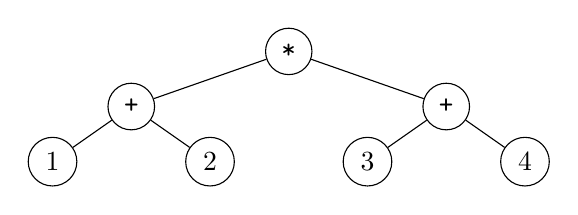
\begin{tikzpicture}[level distance=0.7cm,
    level 1/.style={sibling distance=4cm},
    level 2/.style={sibling distance=2cm},
    level 3/.style={sibling distance=2cm}
    ]
    \node[circle, draw] {\texttt{*}}
      child {node[circle, draw] {\texttt{+}}
        child {node[circle, draw] {1}}
        child {node[circle, draw] {2}}
      }
      child {node[circle, draw] {\texttt{+}}
        child {node[circle, draw] {3}}
        child {node[circle, draw] {4}}
      };
  \end{tikzpicture}
\]

\podnaloga
  Sestavite funkcijo \texttt{izracunaj}, ki izraz evalvira. Na primer:
  \begin{verbatim}
  ghci> izracunaj (Samo 1)
  1
  ghci> izracunaj (Krat (Plus (Samo 1) (Samo 2)) (Samo 3))
  9
  ghci> izracunaj (Krat (Plus (Samo 1) (Samo 2)) (Krat (Samo 3) (Samo 4)))
  36
  \end{verbatim}

\podnaloga
  Podatkovni tip \texttt{Izraz} napravite za primerek razreda tipov \texttt{Num}.
  Vrednosti \texttt{abs}, \texttt{signum} in \texttt{negate} lahko definirate kot \texttt{undefined}.
  \begin{verbatim}
  ghci> 1 + (Samo 2)
  Plus (Samo 1) (Samo 2)
  ghci> (1 + 3) * (Plus (Samo 1) (Samo 2))
  Krat (Plus (Samo 1) (Samo 3)) (Plus (Samo 1) (Samo 2))
  \end{verbatim}

%%%%%%%%%%%%%%%%%%%%%%%%%%%%%%%%%%%%%%%%%%%%%%%%%%%%%%%%%%%%%%%%%%%%%%
\naloga[Fiksne točke, 20 točk]
  Sestavite funkcijo \texttt{fiksna}, ki sprejme urejen seznam celih števil 
  $[x_1, \dots, x_n]$ in v času $O(\log n)$ izračuna najmanjši indeks $i$, za katerega velja $x_i = i$.
  Če tak indeks ne obstaja, naj funkcija vrne \texttt{None} oziroma \texttt{Nothing}.
  Na primer:

  \begin{verbatim}
  >>> fiksna([-4, -2, 0, 2, 4])
  4
  >>> fiksna([-4, -2, 0, 3, 4])
  3
  >>> fiksna([-4, -2, 0, 2, 3])
  None
  \end{verbatim}   
  %
  Nalogo načeloma rešujte v Pythonu, ker boste tako laže dosegli iskano časovno
  zahtevnost. Če želite uporabiti Haskell, namesto seznamov uporabite tabele,
  ki jih ponuja modul \texttt{Data.Array}.

%%%%%%%%%%%%%%%%%%%%%%%%%%%%%%%%%%%%%%%%%%%%%%%%%%%%%%%%%%%%%%%%%%%%%%
\naloga[Orbite, 20 točk]

\podnaloga
  Sestavite funkcijo \texttt{orbita}, ki izračuna seznam vseh različnih
  elementov, ki jih lahko dobimo z zaporedno uporabo dane funkcije na danem
  elementu. Na primer:
  \begin{verbatim}
  ghci> orbita (\x -> mod (x + 2) 10) 13
  [13,5,7,9,1,3]
  ghci> orbita succ 5
  [5,6,7,8,9,10,11,...]
  ghci> orbita negate 0
  [0]
  ghci> orbita negate 1
  [1,-1]
  \end{verbatim}

\podnaloga
  Sestavite funkcijo \texttt{generatorji}, ki izračuna najkrajši seznam vseh
  elementov, ki jih potrebujemo, da z zaporedno uporabo dane funkcije dobimo
  vse elemente danega seznama. Na primer:
  \begin{verbatim}
  ghci> generatorji negate [1,-2,-1]
  [1,-2]
  ghci> generatorji (\x -> (x + 3) `mod` 10) [1,2,3,4]
  [1]
  ghci> generatorji (\x -> (x + 2) `mod` 10) [1,2,3,4]
  [1,2]
  ghci> generatorji (\x -> (x + 2) `mod` 10) [1,2,3,4,5,11]
  [2,11] 
  \end{verbatim}
  Če je najkrajših seznamov več, lahko funkcija vrne katerega koli.


%%%%%%%%%%%%%%%%%%%%%%%%%%%%%%%%%%%%%%%%%%%%%%%%%%%%%%%%%%%%%%%%%%%%%%
\naloga[Vžigalice, 20 točk]

Igralca $A$ in $B$ igrata igro {\em Vžigalice}. Igralca igrata
izmenično, igro prične igrati igralec $A$. Na začetku igre je pred igralcema
kup $n$ vžigalic. Igralec na potezi s kupa odstrani najmanj $3$ vžigalice 
in največ $10$ vžigalic. Izgubi tisti igralec, ki ne more izvesti poteze.

\podnaloga
  Sestavite funkcijo \texttt{kup}, ki za dano število $n$ učinkovito izračuna,
  kateri od igralcev ima zmagovalno strategijo. Na primer:
  \begin{verbatim}
  >>> kup(2)                            ghci> kup 2 
  'B'                                   "B"
  >>> kup(3)                            ghci> kup 3 
  'A'                                   "A"
  >>> kup(11)                           ghci> kup 11 
  'B'                                   "B"
  \end{verbatim}

\podnaloga 
  Igro razširimo tako, da igralca igrata z večimi kupi vžigalic. Igralec
  na potezi si izbere kup in z njega odstrani najmanj $3$ in največ $10$
  vžigalic. Izgubi tisti igralec, ki ne more izvesti poteze. 
  Sestavite funkcijo \texttt{kupi}, ki za dan seznam naravnih števil
  učinkovito izračuna, kateri od igralcev ima zmagovalno strategijo. Na primer:
  \begin{verbatim}
  >>> kupi([11])                        ghci> kupi [11]
  'B'                                   "B"
  >>> kupi([2, 11])                     ghci> kupi [2, 11]
  'A'                                   "A"
  >>> kupi([3, 11])                     ghci> kupi [3, 11]
  'B'                                   "B"
  >>> kupi([2, 3, 11])                  ghci> kupi [2, 3, 11]
  'B'                                   "B"
  \end{verbatim}
%
Nalogo lahko rešujete v Pythonu ali v Haskellu.

\end{document}

